% \section{\core{} Selection Details}
% \label{app:core50-details}

% This appendix gives the full selection definitions behind the simplified objective in the main text. The purpose is reproducibility: the main paper explains why the distillation path is reasonable, while this appendix specifies how the scoring terms, constraints, and audits are computed.

% \subsection{Candidate-200 selection audit}

% Candidate-200 is constructed as a calibration pool after the dual-probe stage. Let $\ell_{i,a}^{id}$ and $\ell_{i,a}^{ood}$ denote clipped log-NMSE for dataset $i$ and algorithm $a$. The two-probe disagreement features are
% \[
% g_i^{id}=\ell_{i,\mathrm{LLMSR}}^{id}-\ell_{i,\mathrm{PySR}}^{id},\qquad
% g_i^{ood}=\ell_{i,\mathrm{LLMSR}}^{ood}-\ell_{i,\mathrm{PySR}}^{ood},
% \]
% \[
% G_i=\frac{|g_i^{id}|+|g_i^{ood}|}{2}.
% \]
% Positive gaps indicate PySR advantage and negative gaps indicate LLM-SR advantage. Candidate-200 is selected from high-$G_i$ tasks, one-sided evaluability tasks, and mid-gap tasks under source-family, subgroup, basename, and advantage-side caps. \Cref{tab:candidate200-selection-audit} reports the realized selection modes.

% \begin{table}[ht]
% \centering
% \small
% \caption{Candidate-200 selection modes. The candidate pool is intentionally high-information rather than a random miniature of \reservoir{}.}
% \label{tab:candidate200-selection-audit}
% \begin{tabular}{llrr}
% \toprule
% Pool & Selection mode & \#Datasets & Mean gap \\
% \midrule
% A & strict high-disagreement & 126 & 31.302 \\
% A & relaxed high-disagreement & 14 & 0.259 \\
% B & one-sided evaluability & 20 & -- \\
% C & mid-gap & 40 & 14.331 \\
% \bottomrule
% \end{tabular}
% \end{table}

% \subsection{Probe-4 selection details}

% The 12-method Candidate-200 calibration stage is summarized at the method level by finite ID/OOD rate, explosion rate, operational stability, discrimination, and dataset coverage. Non-LLM probe candidates are first filtered by execution health, then all feasible four-method panels are scored by
% \[
% \mathrm{Score}(P)=0.20H(P)+0.40F(P)+0.25C(P)+0.15V(P).
% \]
% $H(P)$ averages execution health; $F(P)$ measures how well the panel preserves dataset-informativeness judgments from the larger method panel; $C(P)$ rewards response-space complementarity; and $V(P)$ rewards family/subgroup/difficulty coverage. The final decision also applies taxonomy constraints and excludes methods whose construction role is already used in dual-probe mining or whose behavior depends on LLM/RAG context. This is why the final selected panel is not the NMSE-only top-ranked set.

% \begin{table}[ht]
% \centering
% \small
% \caption{Candidate-200 algorithm health metrics used before Probe-4 subset selection.}
% \label{tab:probe4-health-audit}
% \begin{tabular}{llrrrr}
% \toprule
% Algorithm & Taxonomy & Finite rate & Explosion rate & Stability & Score \\
% \midrule
% PySR & evolutionary-GP & 0.985 & 0.205 & 0.973 & 0.600 \\
% iMCTS & MCTS & 0.990 & 0.055 & 0.990 & 0.481 \\
% uDSR & RL-hybrid & 0.990 & 0.015 & 0.990 & 0.469 \\
% gplearn & classic-GP & 1.000 & 0.140 & 1.000 & 0.449 \\
% TPSR & pretrained-neural & 0.975 & 0.250 & 0.975 & 0.448 \\
% DSO & RL-policy & 0.990 & 0.050 & 0.990 & 0.441 \\
% RAG-SR & RAG-hybrid & 0.885 & 0.585 & 0.885 & 0.415 \\
% PyOperon & evolutionary-GP & 0.975 & 0.035 & 0.967 & 0.369 \\
% E2ESR & pretrained-neural & 0.695 & 0.140 & 0.695 & 0.366 \\
% QLattice & graph-hybrid & 0.950 & 0.030 & 0.950 & 0.361 \\
% \bottomrule
% \end{tabular}
% \end{table}

% \begin{table}[ht]
% \centering
% \small
% \caption{Probe-4 subset audit. The final selected panel is reported alongside the NMSE-only high-scoring panels to make the taxonomy-aware decision explicit.}
% \label{tab:probe4-combination-audit}
% \begin{tabular}{rlrrl}
% \toprule
% NMSE-only rank & Probe combination & Score & Finite rate & Selection note \\
% \midrule
% 1 & iMCTS; PySR; RAG-SR; uDSR & 0.790 & 0.963 & NMSE-only high score \\
% 2 & iMCTS; PySR; RAG-SR; TPSR & 0.783 & 0.959 & NMSE-only high score \\
% 3 & PySR; RAG-SR; TPSR; uDSR & 0.781 & 0.959 & NMSE-only high score \\
% 4 & gplearn; iMCTS; PySR; RAG-SR & 0.773 & 0.965 & NMSE-only high score \\
% 5 & gplearn; PySR; RAG-SR; uDSR & 0.772 & 0.965 & NMSE-only high score \\
% 150 & DSO; iMCTS; PyOperon; uDSR & 0.667 & 0.986 & final selected \\
% \bottomrule
% \end{tabular}
% \end{table}

% \subsection{Run-level cleaning and aggregation}

% Unfinished runs are not treated as invalid runs. A run first receives an outcome class:
% \begin{gather*}
% \{\texttt{valid\_finite},\texttt{valid\_extreme},\texttt{partial},
% \texttt{timeout\_no\_output},\\
% \texttt{invalid},\texttt{system\_error},\texttt{not\_finished}\}.
% \end{gather*}
% Only finished runs with the correct dataset identity are evaluable. Valid extreme-error runs remain valid; their NMSE values are clipped rather than dropped.

% For every run, raw NMSE is mapped to clipped log space:
% \[
% \ell(x)=\mathrm{clip}\left(\log_{10}(\max(x,10^{-12})),-12,12\right).
% \]
% For dataset $i$, probe $p$, and seed set $\mathcal{S}$, the dataset--probe aggregates are:
% \[
% m_{i,p}^{id}=\mathrm{median}_{s\in\mathcal{S}_{valid}}\ell(\mathrm{NMSE}_{i,p,s}^{id}),\qquad
% m_{i,p}^{ood}=\mathrm{median}_{s\in\mathcal{S}_{valid}}\ell(\mathrm{NMSE}_{i,p,s}^{ood}),
% \]
% \[
% \begin{aligned}
% r_{i,p}&=\frac{|\mathcal{S}_{valid}|}{|\mathcal{S}_{evaluable}|},\\
% q_{i,p}^{id}&=\mathrm{IQR}_{s\in\mathcal{S}_{valid}}\ell(\mathrm{NMSE}_{i,p,s}^{id}),\\
% q_{i,p}^{ood}&=\mathrm{IQR}_{s\in\mathcal{S}_{valid}}\ell(\mathrm{NMSE}_{i,p,s}^{ood}).
% \end{aligned}
% \]
% If no valid seed is available for a dataset--probe pair, the pair is excluded from performance medians but contributes to invalid and timeout rates.

% \subsection{Robust normalization}

% All continuous selection features use robust min-max normalization:
% \[
% \mathrm{rmin}(x)=P_5(x),\qquad \mathrm{rmax}(x)=P_{95}(x),
% \]
% \[
% \mathrm{Norm}(x)=
% \mathrm{clip}\left(\frac{x-\mathrm{rmin}(x)}{\mathrm{rmax}(x)-\mathrm{rmin}(x)},0,1\right).
% \]
% If $\mathrm{rmax}(x)=\mathrm{rmin}(x)$, the normalized value is set to zero. Robust normalization prevents a small number of catastrophic NMSE explosions from dominating the selection score.

% \subsection{Dataset-level information score}

% For each dataset $i$, the Probe-4 response vector contains median ID/OOD quality, OOD-ID degradation, valid-output pattern, and seed variability. The discrimination score is
% \[
% \begin{aligned}
% \mathrm{Disc}_i={}&
% 0.35\,\mathrm{Norm}\!\left(\mathrm{Var}_{p}(m_{i,p}^{id})\right)
% +0.35\,\mathrm{Norm}\!\left(\mathrm{Var}_{p}(m_{i,p}^{ood})\right)\\
% &+0.15\,\mathrm{Norm}\!\left(\mathrm{Var}_{p}(m_{i,p}^{ood}-m_{i,p}^{id})\right)
% +0.10\,\mathrm{Norm}\!\left(\mathrm{Mean}_{p<q}|m_{i,p}^{ood}-m_{i,q}^{ood}|\right)\\
% &+0.05\,\mathrm{Norm}\!\left(H(\mathrm{valid\_pattern}_{i,:})\right).
% \end{aligned}
% \]
% The instability score is
% \[
% \begin{aligned}
% \mathrm{Instab}_i=
% {}&0.40\,\mathrm{Mean}_{p}(q_{i,p}^{ood})
% +0.20\,\mathrm{Mean}_{p}(q_{i,p}^{id})
% +0.20\,\mathrm{Max}_{p}(q_{i,p}^{ood})\\
% &+0.10\,\mathrm{invalid\_rate}_i
% +0.10\,\mathrm{timeout\_rate}_i.
% \end{aligned}
% \]
% The stability and information scores are
% \[
% \mathrm{Stab}_i=1-\mathrm{Norm}(\mathrm{Instab}_i),\qquad
% \mathrm{Info}_i=\mathrm{Disc}_i\cdot \mathrm{Stab}_i.
% \]
% Thus, a dataset receives high information only when it separates probes and the separation is not primarily caused by seed noise, invalid outputs, or timeout artifacts.

% \subsection{Difficulty, failure mode, and eligibility}

% Dataset difficulty is computed from the mean ID/OOD quality across valid probes:
% \[
% \mathrm{Difficulty}_i=
% \mathrm{Mean}_{p}\left[\frac{m_{i,p}^{id}+m_{i,p}^{ood}}{2}\right].
% \]
% Datasets are binned into easy, medium, hard, and extreme by robust quantiles, with high invalid or timeout rates allowed to override the bin to extreme. Failure modes are assigned in priority order: incomplete, invalid-prone, one-sided, unstable, OOD-failure, all-struggle, one-method-wins, and all-good. Eligibility is then one of eligible, limited-quota, excluded, or incomplete. Limited-quota datasets are not discarded; they are allowed to enter \core{} only under caps.

% \subsection{Coverage and balance terms}

% For a categorical attribute $a$, let $\mathcal{C}_a(D)$ be the set of categories observed in the full reservoir and $\mathcal{C}_a(S)$ those observed in a subset. Category coverage is
% \[
% \mathrm{Cov}_a(S)=\frac{|\mathcal{C}_a(S)|}{|\mathcal{C}_a(D)|}.
% \]
% Structural coverage averages coverage over family, subgroup, operator group, feature-count bin, sample-count bin, formula-complexity bin, OOD type, and dummy-variable status. Response coverage averages coverage over difficulty bin, failure mode, winner probe, and valid-output pattern:
% \[
% \mathrm{Coverage}(S)=0.6\,\mathrm{StructuralCoverage}(S)+0.4\,\mathrm{ResponseCoverage}(S).
% \]
% Balance measures distributional similarity to the full reservoir. For categorical attribute $a$, let $p_a^S$ and $p_a^D$ be empirical distributions in the subset and the full reservoir. We use total-variation similarity:
% \[
% \mathrm{Sim}_a(S,D)=1-\frac{1}{2}\sum_{c}|p_a^S(c)-p_a^D(c)|.
% \]
% The balance term is a weighted average of $\mathrm{Sim}_a$ over the same structural and response-derived bins.

% \subsection{Full subset objective and hard constraints}

% The full subset score is
% \[
% J(S)=0.45\,\mathrm{Coverage}(S)+0.35\,\frac{1}{|S|}\sum_{i\in S}\mathrm{Info}_i+0.20\,\mathrm{Balance}(S),
% \]
% subject to:
% \[
% |S|=50.
% \]
% The objective is optimized only over feasible subsets. The main hard constraints are:
% \begin{itemize}[leftmargin=*]
%     \item semantic duplicate cap: each semantic duplicate group appears at most once;
%     \item basename cap: no repeated basename in the released \core{} manifest;
%     \item family quota: each family $f$ receives a smoothed quota derived from reservoir frequency,
%     \[
%     t_f=0.6\frac{n_f}{664}+0.4\frac{1}{F},\qquad
%     q_f^{target}=50t_f,
%     \]
%     \[
%     q_f^{min}=\max(1,\lfloor q_f^{target}-1\rfloor),\qquad
%     q_f^{max}=\lceil q_f^{target}+2\rceil;
%     \]
%     \item subgroup concentration cap: no subgroup can dominate the selected subset;
%     \item difficulty quota: easy, medium, hard, and extreme tasks must all be represented;
%     \item limited-quota caps: invalid-prone, one-sided, unstable, and extreme cases are allowed but capped;
%     \item materialization audit: result-derived columns are removed from the released manifest.
% \end{itemize}
% The realized \core{} family counts are 16 LLM-SRBench, 15 SRSD, 9 SRBench 1.0, 3 Nguyen, 2 SRBench2025, 2 Korns, 2 Keijzer, and 1 Vladislavleva. Each selected basename appears once.

% \subsection{Search procedure}

% Selection is implemented as constrained local search:
% \begin{enumerate}[leftmargin=*]
%     \item construct an initial feasible subset using family quotas and high-information eligible datasets;
%     \item repair hard-constraint violations, especially duplicates and over-concentrated subgroups;
%     \item evaluate $J(S)$ for the feasible subset;
%     \item repeatedly propose one-for-one swaps that preserve feasibility;
%     \item accept swaps that improve $J(S)$;
%     \item run multiple random restarts and retain the highest-scoring feasible subset;
%     \item export the frozen manifest and a selection audit report.
% \end{enumerate}
% This procedure is deliberately auditable rather than opaque: the released artifact records the input dataset-level table, selection scores, selected manifest, and post-selection balance report.

% \subsection{Baseline subset definitions}

% We compare \core{} with several 50-task alternatives:
% \begin{itemize}[leftmargin=*]
%     \item \textbf{random-50}: uniformly sampled 50-task subsets;
%     \item \textbf{family-stratified random-50}: random subsets sampled approximately proportional to family sizes;
%     \item \textbf{top-info-50}: top 50 datasets by $\mathrm{Info}_i$;
%     \item \textbf{metadata-diverse-50}: metadata-only diverse subset using feature count, formula complexity, sample count, and family coverage;
%     \item \textbf{difficulty-balanced-50}: quota-balanced subset over difficulty bins, with high-information tie-breaks.
% \end{itemize}
% \Cref{tab:core50-baseline-quality-audit} reports the subset-quality summary used for the radar plot in the main text. Some columns are quality scores where higher is better; the rank-fidelity comparison additionally reports $1-\mathrm{aggregate\ error}$ in the generated figure.

% \begin{table}[ht]
% \centering
% \small
% \caption{Subset-quality summary for \core{} and alternative 50-task selectors. Higher is better for all columns shown here.}
% \label{tab:core50-baseline-quality-audit}
% \resizebox{\linewidth}{!}{%
% \begin{tabular}{lrrrrrr}
% \toprule
% Subset & Coverage & Mean info & Rank fidelity & Stability & Non-red. & Diff. balance \\
% \midrule
% \core{} & 0.838 & 0.471 & 1.000 & 0.835 & 0.769 & 0.892 \\
% top-info-50 & 0.784 & 0.691 & 1.000 & 0.911 & 0.860 & 0.780 \\
% metadata-diverse-50 & 0.635 & 0.085 & 1.000 & 0.735 & 0.860 & 0.601 \\
% difficulty-balanced-50 & 0.817 & 0.637 & 1.000 & 0.883 & 0.920 & 0.999 \\
% random-50 avg & 0.835 & 0.187 & 0.983 & 0.705 & 0.970 & 0.908 \\
% family-stratified random-50 avg & 0.815 & 0.191 & 0.995 & 0.696 & 0.968 & 0.909 \\
% \bottomrule
% \end{tabular}
% }
% \end{table}
\section{\core{} Distillation Details}
\label{app:core50-details}

This appendix provides the full selection definitions behind the simplified \core{} distillation procedure in the main text. The purpose of this appendix is reproducibility and auditability: the main paper explains the rationale of the cascaded distillation path, while this appendix specifies how the scoring terms, constraints, subset baselines, and construction audits are computed.

\subsection{Candidate-200 Selection Audit}
\label{app:candidate200-audit}

Candidate-200 is constructed as a high-information calibration pool after the dual-probe mining stage. The two probes are PySR and LLM-SR, each run once on all 664 ground-truth datasets:$664 \times 2 = 1328.$
%Physical background descriptions are withheld during this stage, so the LLM-based probe cannot directly exploit semantic context.

Let \(\ell_{i,a}^{id}\) and \(\ell_{i,a}^{ood}\) denote clipped log-NMSE for dataset \(i\) and algorithm \(a\) on the ID and OOD test splits. The two-probe disagreement features are
\[
g_i^{id}
=
\ell_{i,\mathrm{LLMSR}}^{id}
-
\ell_{i,\mathrm{PySR}}^{id},
\qquad
g_i^{ood}
=
\ell_{i,\mathrm{LLMSR}}^{ood}
-
\ell_{i,\mathrm{PySR}}^{ood},
\]
and the overall disagreement score is
\[
G_i
=
\frac{
|g_i^{id}|
+
|g_i^{ood}|
}{2},
\]
 here positive gaps indicate PySR advantage, while negative gaps indicate LLM-SR advantage.

Candidate-200 combines high-disagreement tasks, one-sided evaluability cases, and mid-gap tasks under source-family, subgroup, basename, and advantage-side caps. The resulting pool is therefore a calibration set designed to expose method differences and failure modes rather than a random miniature of \reservoir{}.

\begin{table}[ht]
\centering
\small
\caption{\textbf{Candidate-200 selection modes.}}
\label{tab:candidate200-selection-audit}
\begin{tabular}{llrr}
\toprule
\textbf{Pool} & \textbf{Selection mode} & \textbf{\#Datasets} & \textbf{Mean gap} \\
\midrule
A & strict high-disagreement & 126 & 31.302 \\
A & relaxed high-disagreement & 14 & 0.259 \\
B & one-sided evaluability & 20 & -- \\
C & mid-gap & 40 & 14.331 \\
\bottomrule
\end{tabular}
\end{table}

As shown in \Cref{tab:candidate200-selection-audit}, the realized label distribution is 126\ $\mathrm{strict}$,
14\ $\mathrm{relaxed}$,
20\ $\mathrm{one\mbox{-}sided}$,
40\ $\mathrm{mid\mbox{-}gap}$.
The realized family distribution is:
\[
70\ \mathrm{SRSD},
\quad
70\ \mathrm{LLM\mbox{-}SRBench},
\quad
33\ \mathrm{SRBench1.0},
\]
\[
9\ \mathrm{Korns},
\quad
6\ \mathrm{Keijzer},
\quad
6\ \mathrm{Nguyen},
\quad
6\ \mathrm{SRBench2025}.
\]
\Cref{fig:dual-probe-scatter} shows PySR/LLM-SR disagreement on ID and OOD splits. Selected Candidate-200 tasks are concentrated in off-diagonal or asymmetric regions, indicating that the dual-probe stage captures datasets with informative method differences rather than simply sampling the reservoir at random.
\begin{figure}[ht]
\centering
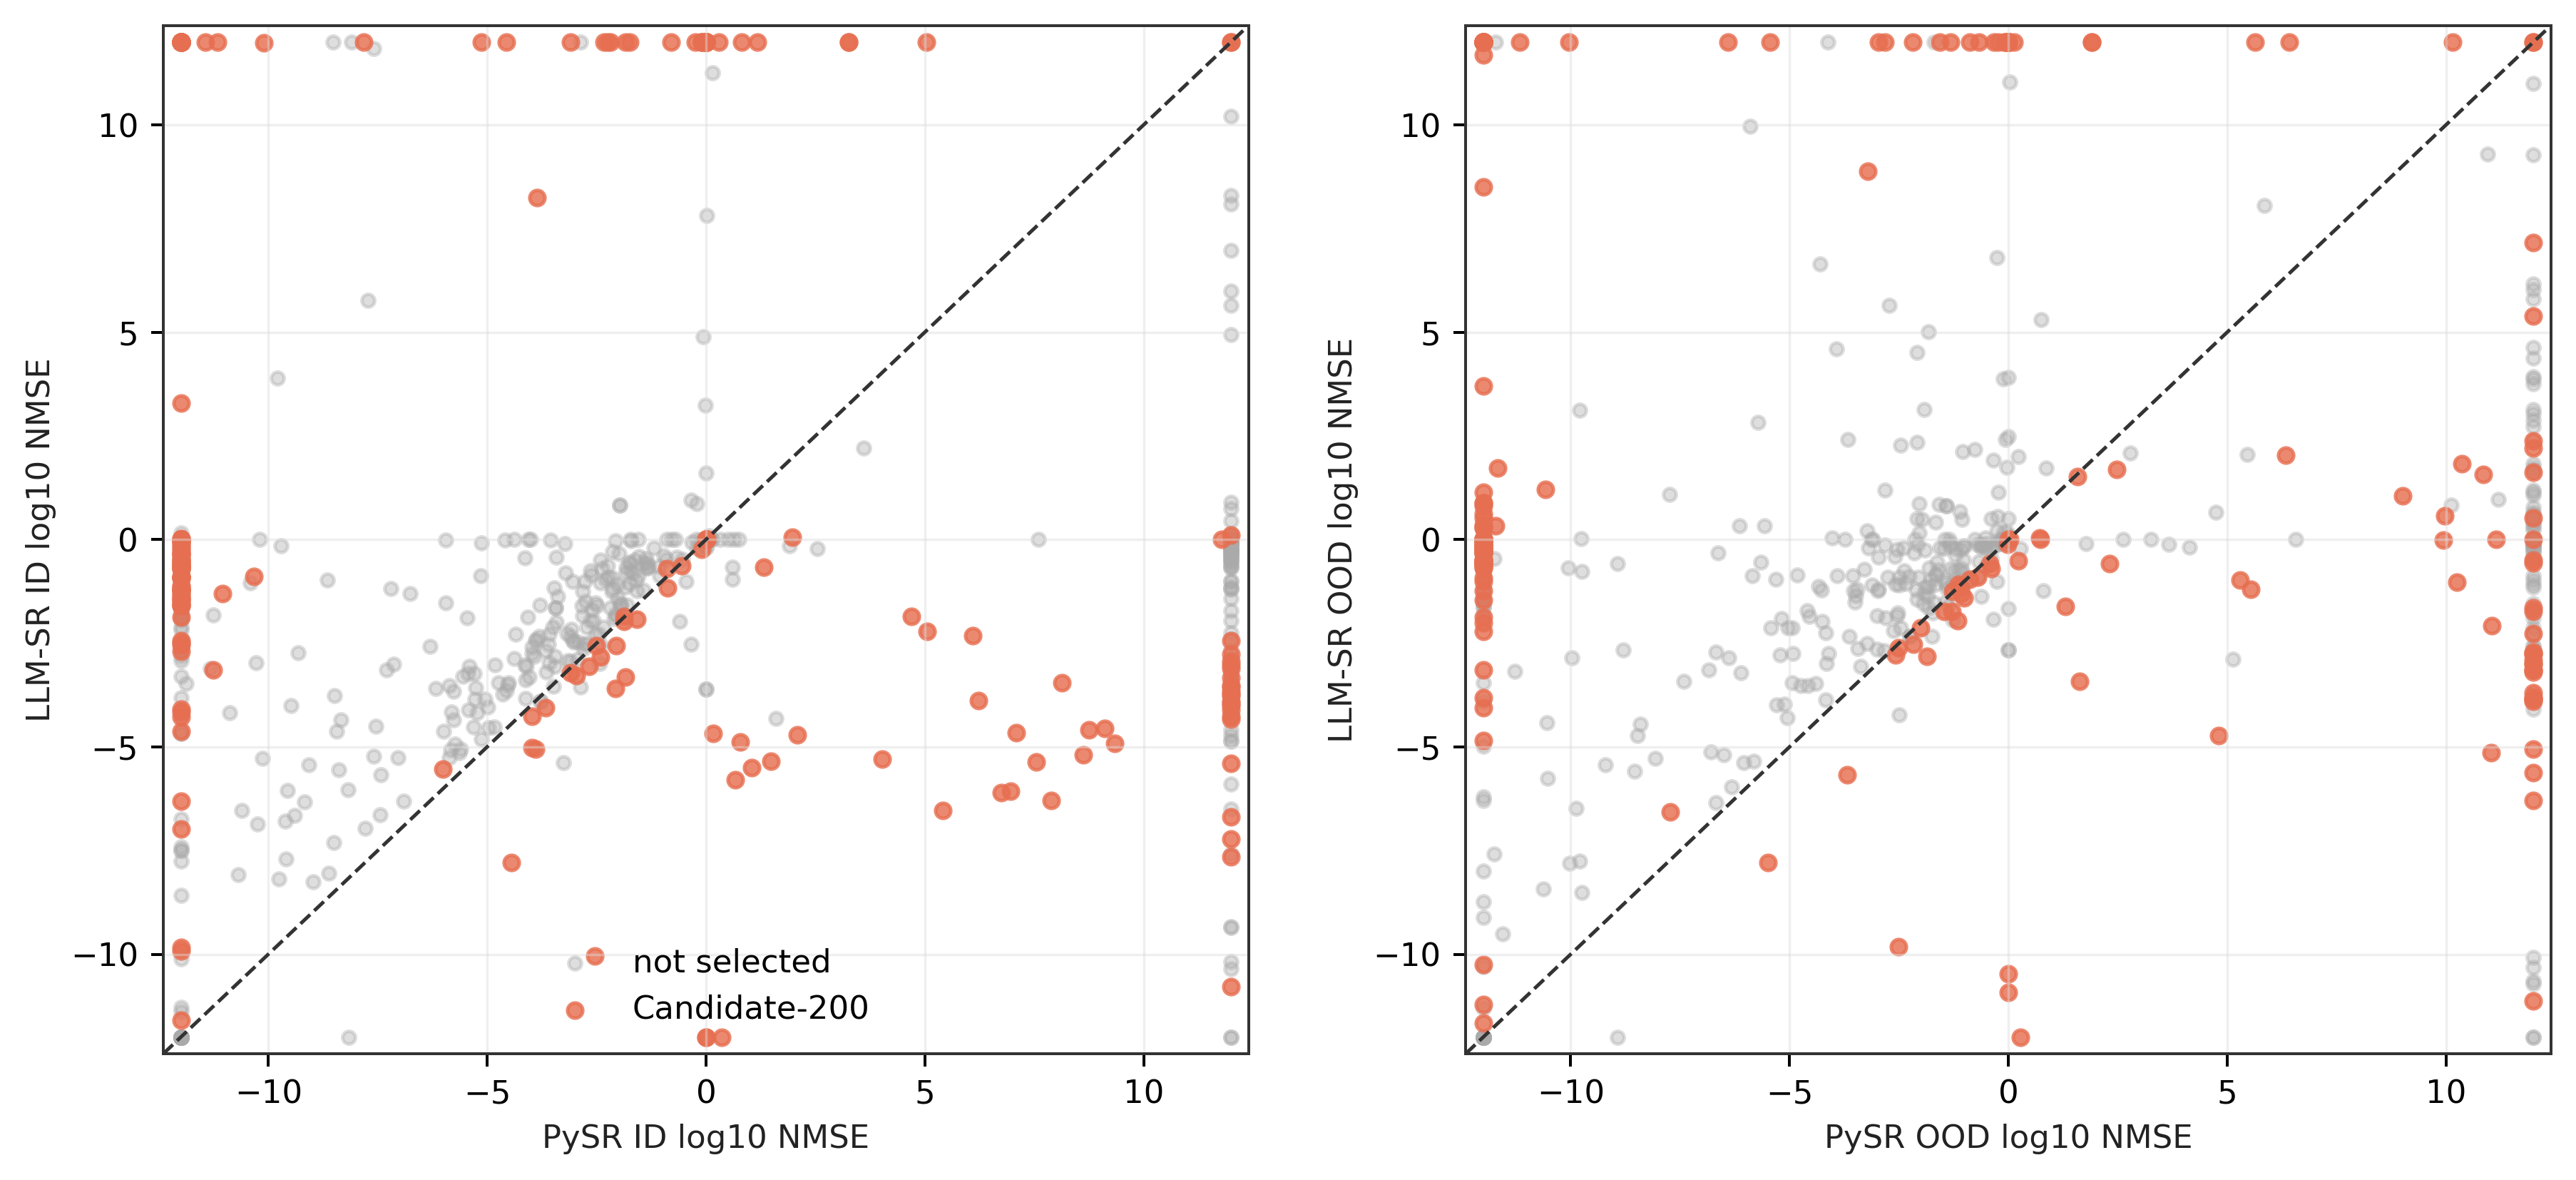
\includegraphics[width=0.68\linewidth]{imgs/Appendix/figure03_dual_probe_scatter}
\caption{\textbf{Dual-probe mining diagnostic.} Each point is a dataset, with PySR and LLM-SR log-NMSE shown on the two axes. Off-diagonal points indicate strong probe disagreement; selected Candidate-200 tasks cover these informative regions on both ID and OOD splits.}
\label{fig:dual-probe-scatter}
\end{figure}


\subsection{Probe-4 Selection Details}
\label{app:probe4-selection}

The Probe-4 selection stage uses the 12-method calibration results on Candidate-200.%: $200 \times 12 = 2400$ single-seed runs. 
Each run provides train, ID, and OOD NMSE values, together with validity and failure status.

\paragraph{Health gate.}
An algorithm \(a\) enters the probe candidate pool only if it satisfies:
\[
\mathrm{finite}(a)\ge 0.90,
\qquad
\mathrm{explode}(a)\le 0.25,
\]
The finite-result rate is
\[
\mathrm{finite}(a)
=
\frac{
\#\{d:\mathrm{train},\mathrm{ID},\mathrm{OOD}\ \mathrm{NMSE\ are\ finite}\}
}{
|D_{\mathrm{cand}}|
},
\]
and the explosion rate is
\[
\mathrm{explode}(a)
=
\frac{
\#\{d:\max(e^{id}_{a,d},e^{ood}_{a,d})>10^2\}
}{
|D_{\mathrm{cand}}|
}.
\]
%Valid extreme-error runs remain valid and are clipped.

\begin{table}[ht]
\centering
\small
\caption{\textbf{Candidate-200 health-gate audit.} This audit is used before Probe-4 subset scoring. The gate is identity-agnostic: LLM-assisted methods are not manually removed, but they fail because their explosion rates exceed the threshold.}
\label{tab:probe4-health-audit}
\begin{tabular}{lrrl}
\toprule
\textbf{Algorithm} & \textbf{Finite rate} & \textbf{Explosion rate} & \textbf{Gate result} \\
\midrule
DSO & 0.990 & 0.050 & pass \\
PyOperon & 0.975 & 0.035 & pass \\
iMCTS & 0.990 & 0.055 & pass \\
uDSR & 0.990 & 0.015 & pass \\
PySR & 0.985 & 0.205 & pass \\
QLattice & 0.950 & 0.030 & pass \\
TPSR & 0.975 & 0.250 & pass \\
gplearn & 1.000 & 0.140 & pass \\
LLM-SR & 1.000 & 0.365 & fail: explosion \\
DRSR & 1.000 & 0.355 & fail: explosion \\
E2ESR & 0.695 & 0.140 & fail: finite \\
RAG-SR & 0.885 & 0.585 & fail: finite/explosion \\
\bottomrule
\end{tabular}
\end{table}

After health filtering, all feasible four-method subsets are enumerated:
\[
P\subset A_{\mathrm{probe}},
\qquad
|P|=4.
\]
The selection also enforces taxonomy diversity:
\[
|\{\mathrm{taxonomy}(a):a\in P\}|\ge 3,
\]
and prevents a single taxonomy from dominating the probe set:
\[
\max_c \#\{a\in P:\mathrm{taxonomy}(a)=c\}\le 2.
\]

\paragraph{Probe-panel score.}
Each feasible panel \(P\) is scored by
\[
\mathrm{Score}(P)
=
0.20H(P)
+
0.40F(P)
+
0.25C(P)
+
0.15V(P).
\]
Here \(H(P)\) is execution health, \(F(P)\) is panel fidelity, \(C(P)\) is behavioral complementarity, and \(V(P)\) is dataset coverage.

Health is defined as
\[
H(P)
=
\frac{1}{|P|}
\sum_{a\in P}
\frac{
\mathrm{finite}(a)+1-\mathrm{explode}(a)
}{2}.
\]

To compute panel fidelity, NMSE values are first transformed into clipped log space:
\[
e^{id}_{i,a}
=
\mathrm{clip}
\left(
\log_{10}(\max(\mathrm{id\_nmse}_{i,a},10^{-12})),
-12,
12
\right),
\]
\[
e^{ood}_{i,a}
=
\mathrm{clip}
\left(
\log_{10}(\max(\mathrm{ood\_nmse}_{i,a},10^{-12})),
-12,
12
\right).
\]
Within each dataset, algorithms are rank-normalized:
\[
s^{id}_{i,a}
=
1-\frac{r^{id}_{i,a}-1}{|A|-1},
\qquad
s^{ood}_{i,a}
=
1-\frac{r^{ood}_{i,a}-1}{|A|-1},
\]
where rank \(1\) is best. The ID-to-OOD behavior change is
\[
g_{i,a}=s^{ood}_{i,a}-s^{id}_{i,a}.
\]

The full-panel dataset informativeness is
\[
I^{12}(d_i)
=
\mathrm{Var}_{a\in A}(s^{id}_{i,a})
+
\mathrm{Var}_{a\in A}(s^{ood}_{i,a}),
\]
and the informativeness induced by panel \(P\) is
\[
I^P(d_i)
=
\mathrm{Var}_{a\in P}(s^{id}_{i,a})
+
\mathrm{Var}_{a\in P}(s^{ood}_{i,a}).
\]
Panel fidelity is
\[
F(P)
=
\frac{1+\rho_{\mathrm{Spearman}}(I^P,I^{12})}{2}.
\]

Behavioral complementarity is computed from the algorithm behavior vector
\[
z_a=
[
s^{id}_{1,a},\ldots,s^{id}_{200,a},
s^{ood}_{1,a},\ldots,s^{ood}_{200,a},
g_{1,a},\ldots,g_{200,a}
].
\]
The pairwise behavior distance is
\[
D(a,b)
=
\frac{1-\rho_{\mathrm{Spearman}}(z_a,z_b)}{2},
\]
and the complementarity score is
\[
C(P)
=
\frac{2}{|P|(|P|-1)}
\sum_{a<b,\ a,b\in P}D(a,b).
\]

Dataset coverage is computed from the Top-50 datasets ranked by \(I^P\):
\[
T^P_{50}
=
\mathrm{Top50}_{d_i} I^P(d_i).
\]
It combines family and subgroup coverage:
\[
V(P)
=
0.5V_{\mathrm{family}}(P)
+
0.5V_{\mathrm{subgroup}}(P),
\]
with the hard constraint
\[
\max_f
\frac{
\#\{d_i\in T^P_{50}:\mathrm{family}(d_i)=f\}
}{50}
\le 0.40.
\]

\begin{table}[ht]
\centering
\small
\caption{\textbf{Probe-4 candidate-panel audit.} The first five rows are comparable health-gated panels. Finite-only and no-health-gate rows are included to show that LLM panels are not top choices under finite-only relaxation, and that removing the health gate lets missing-output and explosion artifacts dominate.}
\label{tab:probe4-combination-audit}
\resizebox{\linewidth}{!}{%
\begin{tabular}{llrl}
\toprule
\textbf{Audit setting} & \textbf{Probe panel} & \textbf{Score} & \textbf{Decision} \\
\midrule
Health-gated rank 1 & DSO; PyOperon; QLattice; uDSR & 0.6570 & strict score optimum \\
\textbf{Health-gated rank 2} & \textbf{DSO; iMCTS; PyOperon; uDSR} & \textbf{0.6512} & \textbf{selected: near tie; adds MCTS/tree search} \\
Health-gated rank 3 & DSO; gplearn; iMCTS; uDSR & 0.6482 & close, but weaker evolutionary-GP coverage \\
Health-gated rank 4 & DSO; gplearn; PySR; TPSR & 0.6454 & high score, but no explicit MCTS probe \\
Health-gated rank 5 & DSO; gplearn; iMCTS; PySR & 0.6407 & lower panel fidelity than selected panel \\
Finite-only rank 7 & DRSR; gplearn; PySR; TPSR & 0.6374 & LLM-assisted panel enters only after Top-5 \\
Finite-only rank 9 & gplearn; LLM-SR; PySR; TPSR & 0.6191 & LLM-SR remains below health-gated alternatives \\
No health gate & E2ESR; PySR; QLattice; RAG-SR & 0.6817 & rejected: missing/explosion artifacts dominate \\
\bottomrule
\end{tabular}
}
\end{table}

As shown in \Cref{tab:probe4-combination-audit}, the final selected panel is
\[
P^*
=
\{
\mathrm{DSO},
\mathrm{PyOperon},
\mathrm{iMCTS},
\mathrm{uDSR}
\}.
\]
It spans RL/policy search, evolutionary GP, MCTS/tree search, and neural-guided SR, serving as a compact surrogate selected under health, taxonomy, and construction-role constraints.

\begin{figure}[ht]
\centering
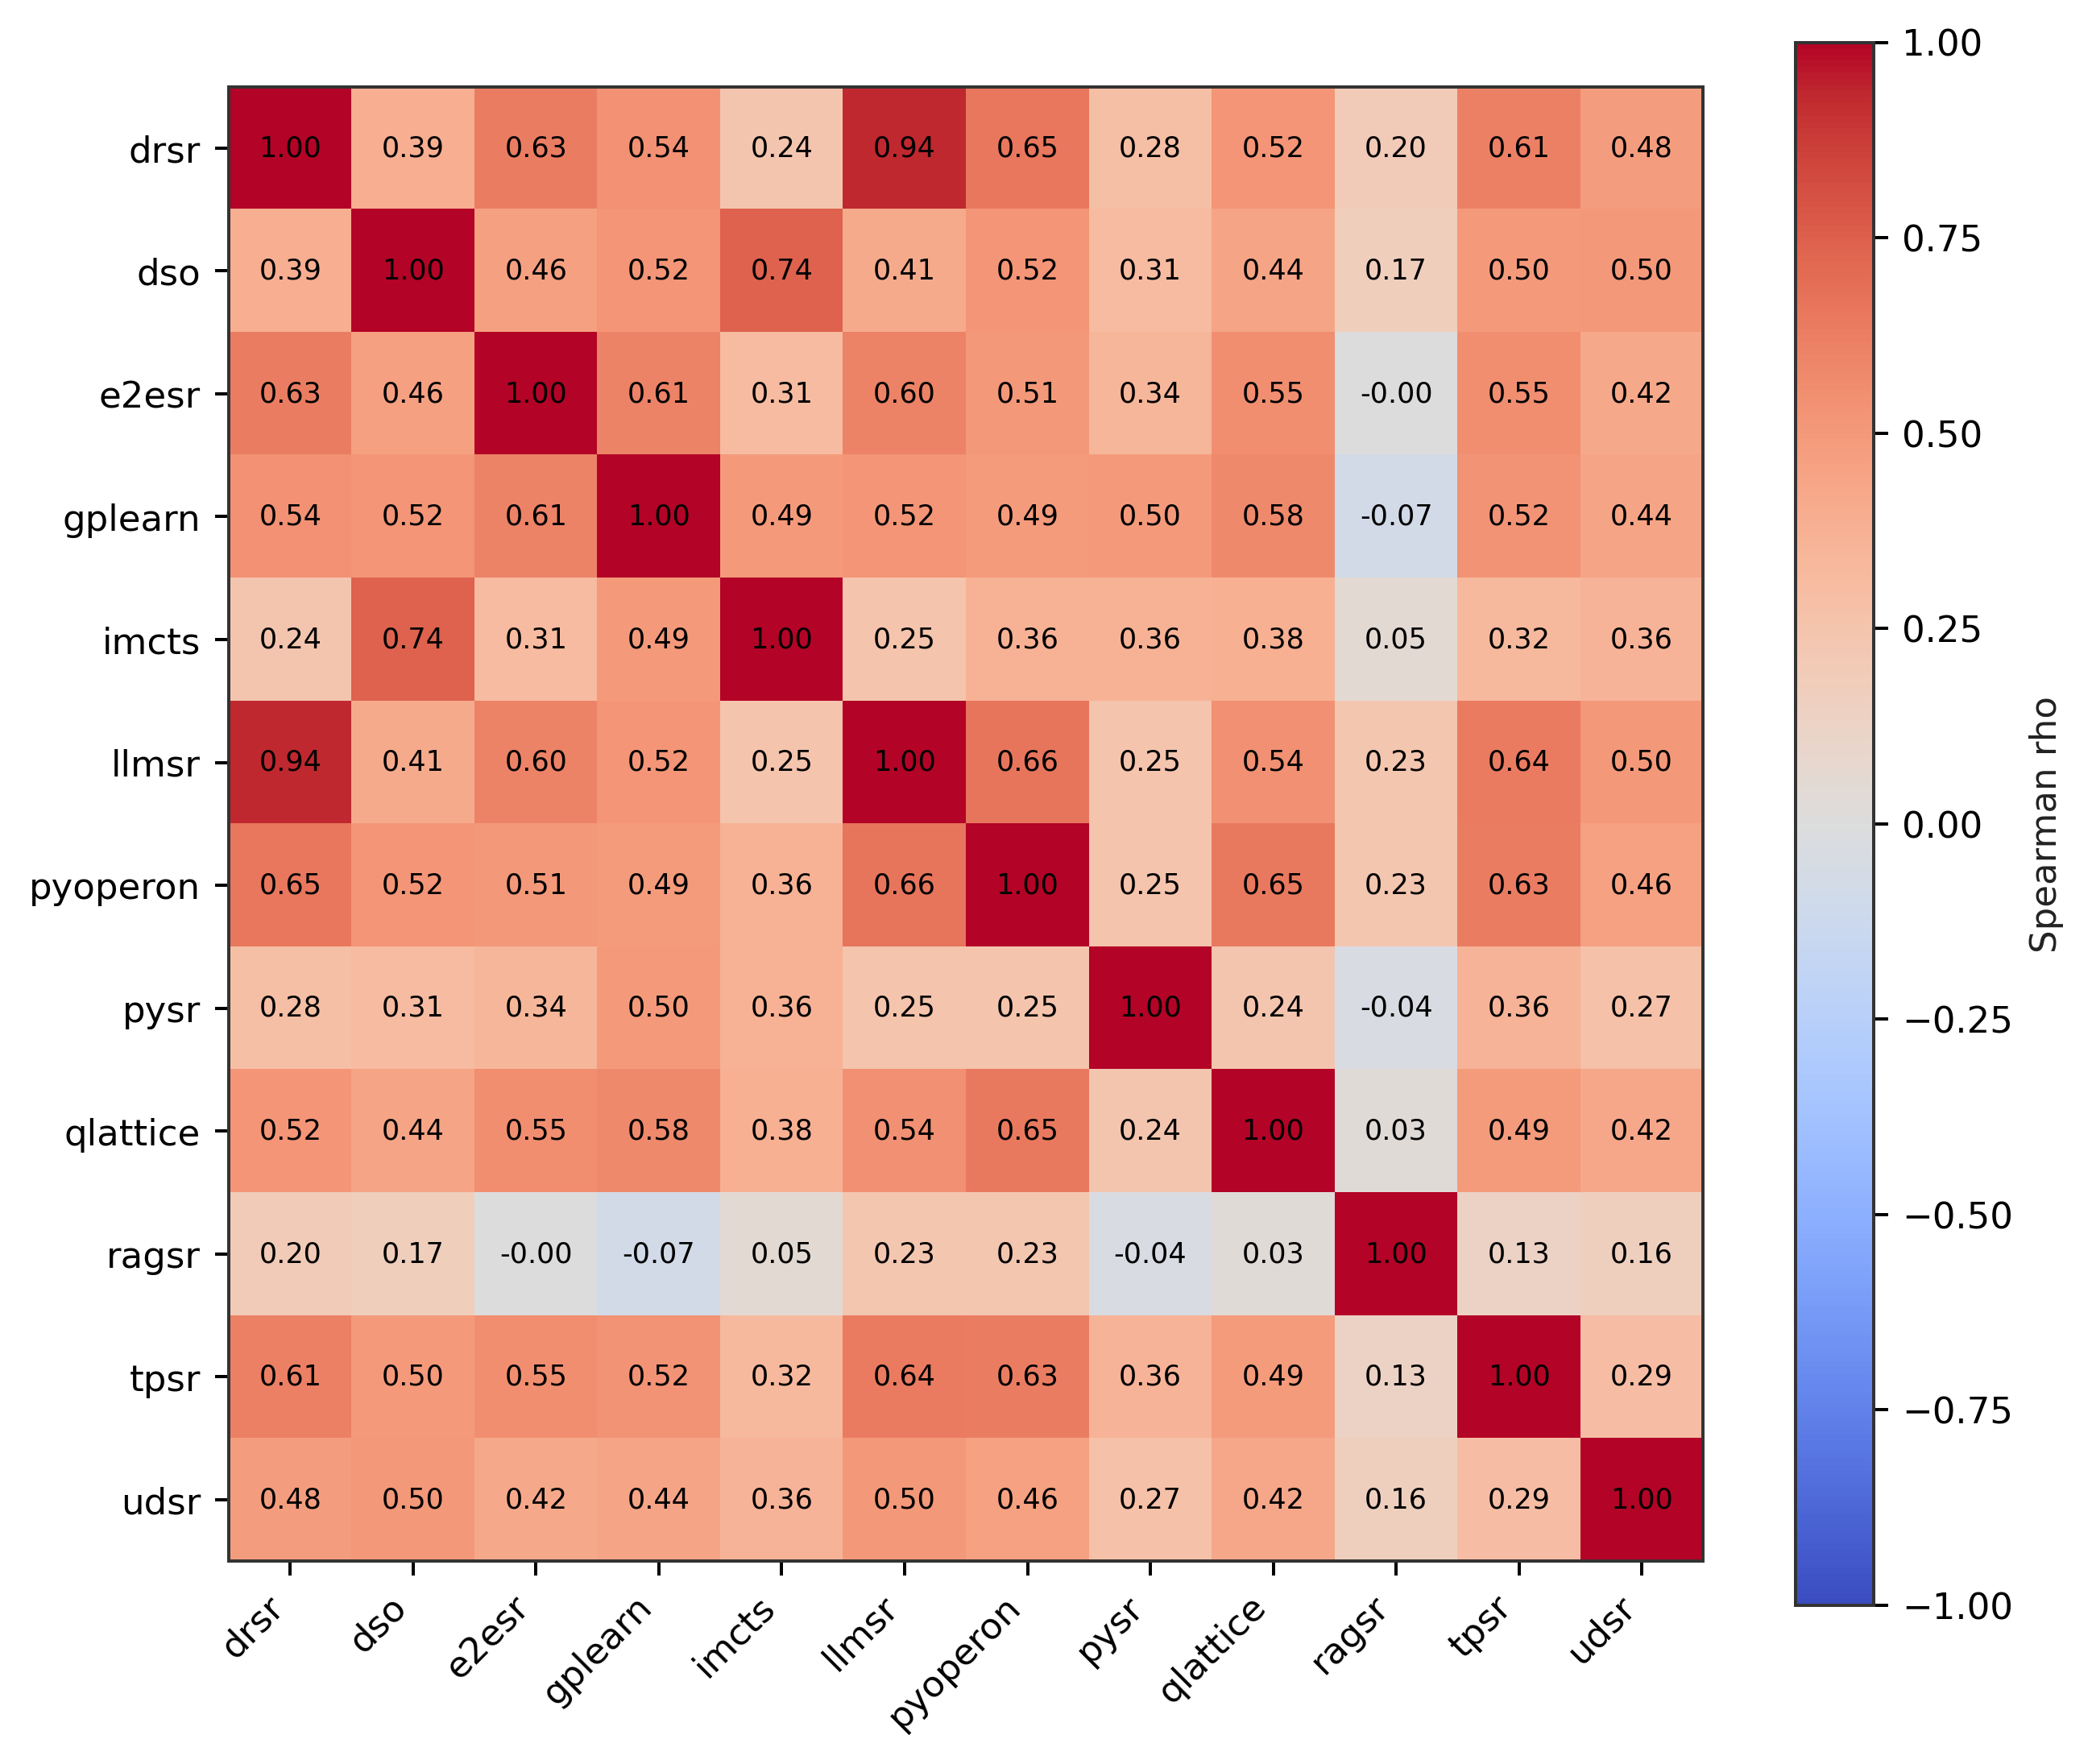
\includegraphics[width=0.68\linewidth]{imgs/Article/figure07_algorithm_behavior_correlation}
\caption{\textbf{Algorithm behavior correlation on Candidate-200.} The correlation structure is used to avoid selecting redundant probes.}
\label{fig:algorithm-behavior-correlation}
\end{figure}


\subsection{Probe4-Full Run Cleaning and Aggregation}
\label{app:probe4-run-cleaning}

The selected Probe-4 is evaluated on all 664 reservoir tasks with three seeds:
\[
664 \times 4 \times 3 = 7968.
\]
Each run records:
\[
\mathrm{dataset\_id},\ 
\mathrm{algorithm},\ 
\mathrm{seed},\ 
\mathrm{status},\ 
\mathrm{valid\_output},
\]
\[
e^{id},\ 
e^{ood},\ 
\mathrm{runtime},\ 
\mathrm{expression},\ 
\mathrm{complexity},\ 
\mathrm{failure\_reason}.
\]

Unfinished runs are not automatically treated as invalid runs. Each run first receives an outcome class:
\[
\{
\texttt{valid\_finite},
\texttt{valid\_extreme},
\texttt{partial},
\texttt{timeout\_no\_output},
\]
\[
\texttt{invalid},
\texttt{system\_error},
\texttt{not\_finished}
\}.
\]
Only finished runs with the correct dataset identity are evaluable. Valid extreme-error runs remain valid, and their NMSE values are clipped rather than dropped.

For every run, raw NMSE is mapped to clipped log space:
\[
\ell(x)
=
\mathrm{clip}
\left(
\log_{10}(\max(x,10^{-12})),
-12,
12
\right).
\]
For dataset \(i\), probe \(p\), and seed set \(\mathcal{S}\), the dataset--probe aggregates are:
\[
m_{i,p}^{id}
=
\mathrm{median}_{s\in\mathcal{S}_{valid}}
\ell(\mathrm{NMSE}_{i,p,s}^{id}),
\]
\[
m_{i,p}^{ood}
=
\mathrm{median}_{s\in\mathcal{S}_{valid}}
\ell(\mathrm{NMSE}_{i,p,s}^{ood}),
\]
\[
r_{i,p}
=
\frac{|\mathcal{S}_{valid}|}{|\mathcal{S}_{evaluable}|},
\]
\[
q_{i,p}^{id}
=
\mathrm{IQR}_{s\in\mathcal{S}_{valid}}
\ell(\mathrm{NMSE}_{i,p,s}^{id}),
\]
\[
q_{i,p}^{ood}
=
\mathrm{IQR}_{s\in\mathcal{S}_{valid}}
\ell(\mathrm{NMSE}_{i,p,s}^{ood}).
\]
If no valid seed is available for a dataset--probe pair, the pair is excluded from performance medians but contributes to invalid and timeout rates.


\subsection{Robust Normalization}
\label{app:robust-normalization}

All continuous selection features use robust min-max normalization:
\[
\mathrm{rmin}(x)=P_5(x),
\qquad
\mathrm{rmax}(x)=P_{95}(x),
\]
\[
\mathrm{Norm}(x)
=
\mathrm{clip}
\left(
\frac{x-\mathrm{rmin}(x)}
{\mathrm{rmax}(x)-\mathrm{rmin}(x)},
0,
1
\right).
\]
If \(\mathrm{rmax}(x)=\mathrm{rmin}(x)\), the normalized value is set to zero. Robust normalization prevents a small number of catastrophic NMSE explosions from dominating the selection score.


\subsection{Dataset-Level Information Score}
\label{app:dataset-information-score}

For each dataset \(i\), the Probe-4 response vector contains median ID/OOD quality, OOD-ID degradation, valid-output pattern, and seed variability. The discrimination score is
\[
\begin{aligned}
\mathrm{Disc}_i
={}&
0.35\,\mathrm{Norm}\!\left(\mathrm{Var}_{p}(m_{i,p}^{id})\right)
+
0.35\,\mathrm{Norm}\!\left(\mathrm{Var}_{p}(m_{i,p}^{ood})\right)\\
&+
0.15\,\mathrm{Norm}\!\left(\mathrm{Var}_{p}(m_{i,p}^{ood}-m_{i,p}^{id})\right)
+
0.10\,\mathrm{Norm}\!\left(\mathrm{Mean}_{p<q}|m_{i,p}^{ood}-m_{i,q}^{ood}|\right)\\
&+
0.05\,\mathrm{Norm}\!\left(H(\mathrm{valid\_pattern}_{i,:})\right).
\end{aligned}
\]
The instability score is
\[
\begin{aligned}
\mathrm{Instab}_i
={}&
0.40\,\mathrm{Mean}_{p}(q_{i,p}^{ood})
+
0.20\,\mathrm{Mean}_{p}(q_{i,p}^{id})
+
0.20\,\mathrm{Max}_{p}(q_{i,p}^{ood})\\
&+
0.10\,\mathrm{invalid\_rate}_i
+
0.10\,\mathrm{timeout\_rate}_i.
\end{aligned}
\]
The stability and information scores are
\[
\mathrm{Stab}_i
=
1-\mathrm{Norm}(\mathrm{Instab}_i),
\qquad
\mathrm{Info}_i
=
\mathrm{Disc}_i\cdot \mathrm{Stab}_i.
\]
Thus, a dataset receives high information only when it separates probes and the separation is not primarily caused by seed noise, invalid outputs, or timeout artifacts.


\subsection{Difficulty, Failure Mode, and Eligibility}
\label{app:difficulty-failure-eligibility}

Dataset difficulty is computed from the mean ID/OOD response across valid probes:
\[
\mathrm{Difficulty}_i
=
\mathrm{Mean}_{p}
\left[
\frac{
m_{i,p}^{id}
+
m_{i,p}^{ood}
}{2}
\right].
\]
Datasets are binned into easy, medium, hard, and extreme by robust quantiles. High invalid or timeout rates are allowed to override the bin to extreme.

Failure modes are assigned in priority order:
\[
\mathrm{incomplete},
\quad
\mathrm{invalid\mbox{-}prone},
\quad
\mathrm{one\mbox{-}sided},
\quad
\mathrm{unstable},
\]
\[
\mathrm{OOD\mbox{-}failure},
\quad
\mathrm{all\mbox{-}struggle},
\quad
\mathrm{one\mbox{-}method\mbox{-}wins},
\quad
\mathrm{all\mbox{-}good}.
\]
Eligibility is one of:
\[
\mathrm{eligible},
\quad
\mathrm{limited\mbox{-}quota},
\quad
\mathrm{excluded},
\quad
\mathrm{incomplete}.
\]
Limited-quota datasets are not discarded; they are allowed to enter \core{} only under explicit caps.


\subsection{Coverage and Balance Terms}
\label{app:coverage-balance}

For a categorical attribute \(a\), let \(\mathcal{C}_a(D)\) be the set of categories observed in the full reservoir and \(\mathcal{C}_a(S)\) those observed in a subset. Category coverage is
\[
\mathrm{Cov}_a(S)
=
\frac{
|\mathcal{C}_a(S)|
}{
|\mathcal{C}_a(D)|
}.
\]
Structural coverage averages coverage over family, subgroup, operator group, feature-count bin, sample-count bin, formula-complexity bin, OOD type, and dummy-variable status. Response coverage averages coverage over difficulty bin, failure mode, winner probe, and valid-output pattern:
\[
\mathrm{Coverage}(S)
=
0.6\,\mathrm{StructuralCoverage}(S)
+
0.4\,\mathrm{ResponseCoverage}(S).
\]

Balance measures distributional similarity to the full reservoir. For categorical attribute \(a\), let \(p_a^S\) and \(p_a^D\) be empirical distributions in the subset and the full reservoir. Total-variation similarity is
\[
\mathrm{Sim}_a(S,D)
=
1
-
\frac{1}{2}
\sum_c
|p_a^S(c)-p_a^D(c)|.
\]
The balance term is a weighted average of \(\mathrm{Sim}_a\) over structural and response-derived bins.


\subsection{Full Subset Objective and Hard Constraints}
\label{app:core50-objective-constraints}

The full subset score is
\[
J(S)
=
0.45\,\mathrm{Coverage}(S)
+
0.35\,\frac{1}{|S|}
\sum_{i\in S}\mathrm{Info}_i
+
0.20\,\mathrm{Balance}(S),
\]
subject to
\[
|S|=50.
\]
The objective is optimized only over feasible subsets. The main hard constraints are:
\begin{itemize}[leftmargin=*]
    \item semantic duplicate cap: each semantic duplicate group appears at most once;
    \item basename cap: no repeated basename in the released \core{} manifest;
    \item family quota: each family \(f\) receives a smoothed quota derived from reservoir frequency;
    \item subgroup concentration cap: no subgroup can dominate the selected subset;
    \item difficulty quota: easy, medium, hard, and extreme tasks must all be represented;
    \item limited-quota caps: invalid-prone, one-sided, unstable, and extreme cases are allowed but capped;
    \item materialization audit: result-derived columns are removed from the released manifest.
\end{itemize}

No source family receives a hand-written special rule. Let \(n_f\) be the number of reservoir tasks in family \(f\), and let \(F\) be the number of families. The smoothed target mass is
\[
t_f
=
0.6\frac{n_f}{664}
+
0.4\frac{1}{F}.
\]
The target count is
\[
q_f^{target}
=
50t_f,
\]
and the lower and upper quota bounds are
\[
q_f^{min}
=
\max(1,\lfloor q_f^{target}-1\rfloor),
\qquad
q_f^{max}
=
\lceil q_f^{target}+2\rceil.
\]
This allocation gives larger families more capacity, prevents smaller families from disappearing, and avoids domination by any single source family.

The realized \core{} family counts are:
\[
16\ \mathrm{LLM\mbox{-}SRBench},
\quad
15\ \mathrm{SRSD},
\quad
9\ \mathrm{SRBench1.0},
\]
\[
3\ \mathrm{Nguyen},
\quad
2\ \mathrm{SRBench2025},
\quad
2\ \mathrm{Korns},
\quad
2\ \mathrm{Keijzer},
\quad
1\ \mathrm{Vladislavleva}.
\]
Each selected basename appears once.


\subsection{Search Procedure}
\label{app:core50-search}

Selection is implemented as constrained local search:
\begin{enumerate}[leftmargin=*]
    \item construct an initial feasible subset using family quotas and high-information eligible datasets;
    \item repair hard-constraint violations, especially duplicates and over-concentrated subgroups;
    \item evaluate \(J(S)\) for the feasible subset;
    \item repeatedly propose one-for-one swaps that preserve feasibility;
    \item accept swaps that improve \(J(S)\);
    \item run multiple random restarts and retain the highest-scoring feasible subset;
    \item export the frozen manifest and a selection audit report.
\end{enumerate}

This procedure is deliberately auditable rather than opaque. The released artifact records the input dataset-level table, selection scores, selected manifest, and post-selection balance report.


\subsection{Baseline Subset Definitions}
\label{app:baseline-selectors}

\core{} is compared with several 50-task alternatives:
\begin{itemize}[leftmargin=*]
    \item \textbf{random-50}: uniformly sampled 50-task subsets;
    \item \textbf{family-stratified random-50}: random subsets sampled approximately proportional to family sizes;
    \item \textbf{top-info-50}: top 50 datasets by \(\mathrm{Info}_i\);
    \item \textbf{metadata-diverse-50}: metadata-only diverse subset using feature count, formula complexity, sample count, and family coverage;
    \item \textbf{response-medoids-50}: response-space medoids in the four-probe ID/OOD/validity/stability feature space;
    \item \textbf{difficulty-balanced-50}: quota-balanced subset over difficulty bins, with high-information tie-breaks.
\end{itemize}


\subsection{Validation Diagnostics}
\label{app:core50-validation-diagnostics}

The validation compares \core{} and alternative 50-task selectors using:
\[
\mathrm{Coverage},
\quad
\mathrm{MeanInfo},
\quad
\mathrm{RankFidelity},
\quad
\mathrm{Stability},
\quad
\mathrm{NonRedundancy},
\quad
\mathrm{DifficultyBalance}.
\]
These columns are diagnostic criteria rather than independent optimization targets. \core{} is selected for their constrained trade-off together with hard feasibility constraints.

\begin{table}[ht]
\centering
\small
\caption{\textbf{Subset-quality summary for \core{} and alternative 50-task selectors.} Higher is better within each diagnostic column, but \core{} is selected for a constrained trade-off rather than for optimizing any single column.}
\label{tab:core50-baseline-quality-audit}
\resizebox{\linewidth}{!}{%
\begin{tabular}{lrrrrrr}
\toprule
Subset & Coverage & Mean info & Rank fidelity & Stability & Non-red. & Diff. balance \\
\midrule
\core{} & 0.838 & 0.471 & 1.000 & 0.835 & 0.769 & 0.892 \\
top-info-50 & 0.784 & 0.691 & 1.000 & 0.911 & 0.860 & 0.780 \\
metadata-diverse-50 & 0.635 & 0.085 & 1.000 & 0.735 & 0.860 & 0.601 \\
difficulty-balanced-50 & 0.817 & 0.637 & 1.000 & 0.883 & 0.920 & 0.999 \\
random-50 avg & 0.835 & 0.187 & 0.983 & 0.705 & 0.970 & 0.908 \\
family-stratified random-50 avg & 0.815 & 0.191 & 0.995 & 0.696 & 0.968 & 0.909 \\
\bottomrule
\end{tabular}
}
\end{table}

\subsection{Release and Leakage Control}
\label{app:core50-release-leakage}

After validation, \core{} is frozen as the official benchmark subset. Probe4-Full results are used only for benchmark construction. The final leaderboard is recomputed independently by running all 12 algorithms on frozen \core{} with five seeds:$12\times 50\times 5 = 3000.$

The released \core{} manifest contains dataset identity and static metadata needed for benchmark materialization. It excludes result-derived columns such as probe gap, priority score, selected advantage side, Probe-4 informativeness score, and selection rank. This prevents downstream methods from directly exploiting construction signals.

The frozen benchmark release includes:
\[
\mathrm{core50\_v1.json},
\qquad
\mathrm{core50\_metadata.csv},
\qquad
\mathrm{core50\_selection\_report.pdf}.
\]

\Cref{tab:core50-ablation-summary} reports the subset-quality summary used for the main-text validation table. The composite objective summarizes the coverage--information--stability trade-off, while aggregate-score MAE measures fidelity to the full 664-task reservoir. The important empirical pattern is that single-axis selectors can improve one summary dimension, but they lose substantially more full-reservoir fidelity than \core{}.

\begin{table}[t]
\centering
\small
\caption{\textbf{Core-50 ablation against deterministic and random 50-task selectors.} Higher is better for objective score, coverage, mean information, and mean stability; lower is better for aggregate-score MAE.}
\label{tab:core50-ablation-summary}
\resizebox{\linewidth}{!}{%
\begin{tabular}{lrrrrr}
\toprule
\textbf{Selector} & \textbf{Objective} & \textbf{Coverage} & \textbf{Mean info} & \textbf{Mean stability} & \textbf{Agg. MAE} \\
\midrule
Random avg & 0.6157 & \textbf{0.7804} & 0.1949 & 0.7070 & 0.4949 \\
Family-random avg & 0.6105 & 0.7772 & 0.1910 & 0.6912 & 0.5243 \\
Metadata-diverse & 0.6744 & 0.7712 & 0.3738 & 0.8340 & 0.5060 \\
Response-space K-medoids & 0.6342 & 0.7660 & 0.2726 & 0.6258 & 0.6044 \\
Top-information & \textbf{0.7305} & 0.7216 & \textbf{0.6049} & 0.8931 & 1.0339 \\
Difficulty-balanced & 0.6957 & 0.7122 & 0.5145 & 0.8375 & 1.0430 \\
\core{} & 0.7284 & 0.7736 & 0.5308 & \textbf{0.8997} & \textbf{0.1388} \\
\bottomrule
\end{tabular}
}
\end{table}

